\section{Cahier des charges}
Cette partie présente le cahier des charges du périphérique.
Elle intègre les quelques points fournis par le sujet auquel s'ajoutent les contraintes imaginées par les étudiants.
\subsection{Objectif du circuit}
Le contrôleur d'interruptions a pour rôle d'informer le processeur sur l’occurrence d'une interruption valide.
Il fournira alors l’adresse de la prochaine instruction à exécuter.

\subsection{Fonctionnalités attendues}
Les fonctions de service du circuit sont :
\begin{enumerate}
    \item Masquer et démasquer chaque interruption individuellement
    \item Contenir et permettre la configuration du vecteur d'exception
    \item Permettre de configurer la priorité des interruptions
    \item Ne fournir au \gls{CPU} que les interruptions valides
    \item Prendre en compte les priorités dans la génération des demandes au \gls{CPU}
\end{enumerate}
\subsection{Utilisation du circuit}
	
Il s'agit ici de donner l'utilisation du circuit en présentant le schéma de câblage du contrôleur d'interruptions ainsi que la définition des signaux logiques d'entrées et sorties.
L'\gls{IP} à concevoir s'interface avec le bus de données, le bus d'adresses ainsi qu'un ensemble de signaux de temporisation et de contrôle.
Il est possible de retrouver des signaux de temporisation comme le nWAIT et des signaux de contrôle comme le nRST ou le RnW.
Leur rôle est présenté table (\ref{tab:sens_role_signaux}).
	
\begin{figure}[H]
	\centering
	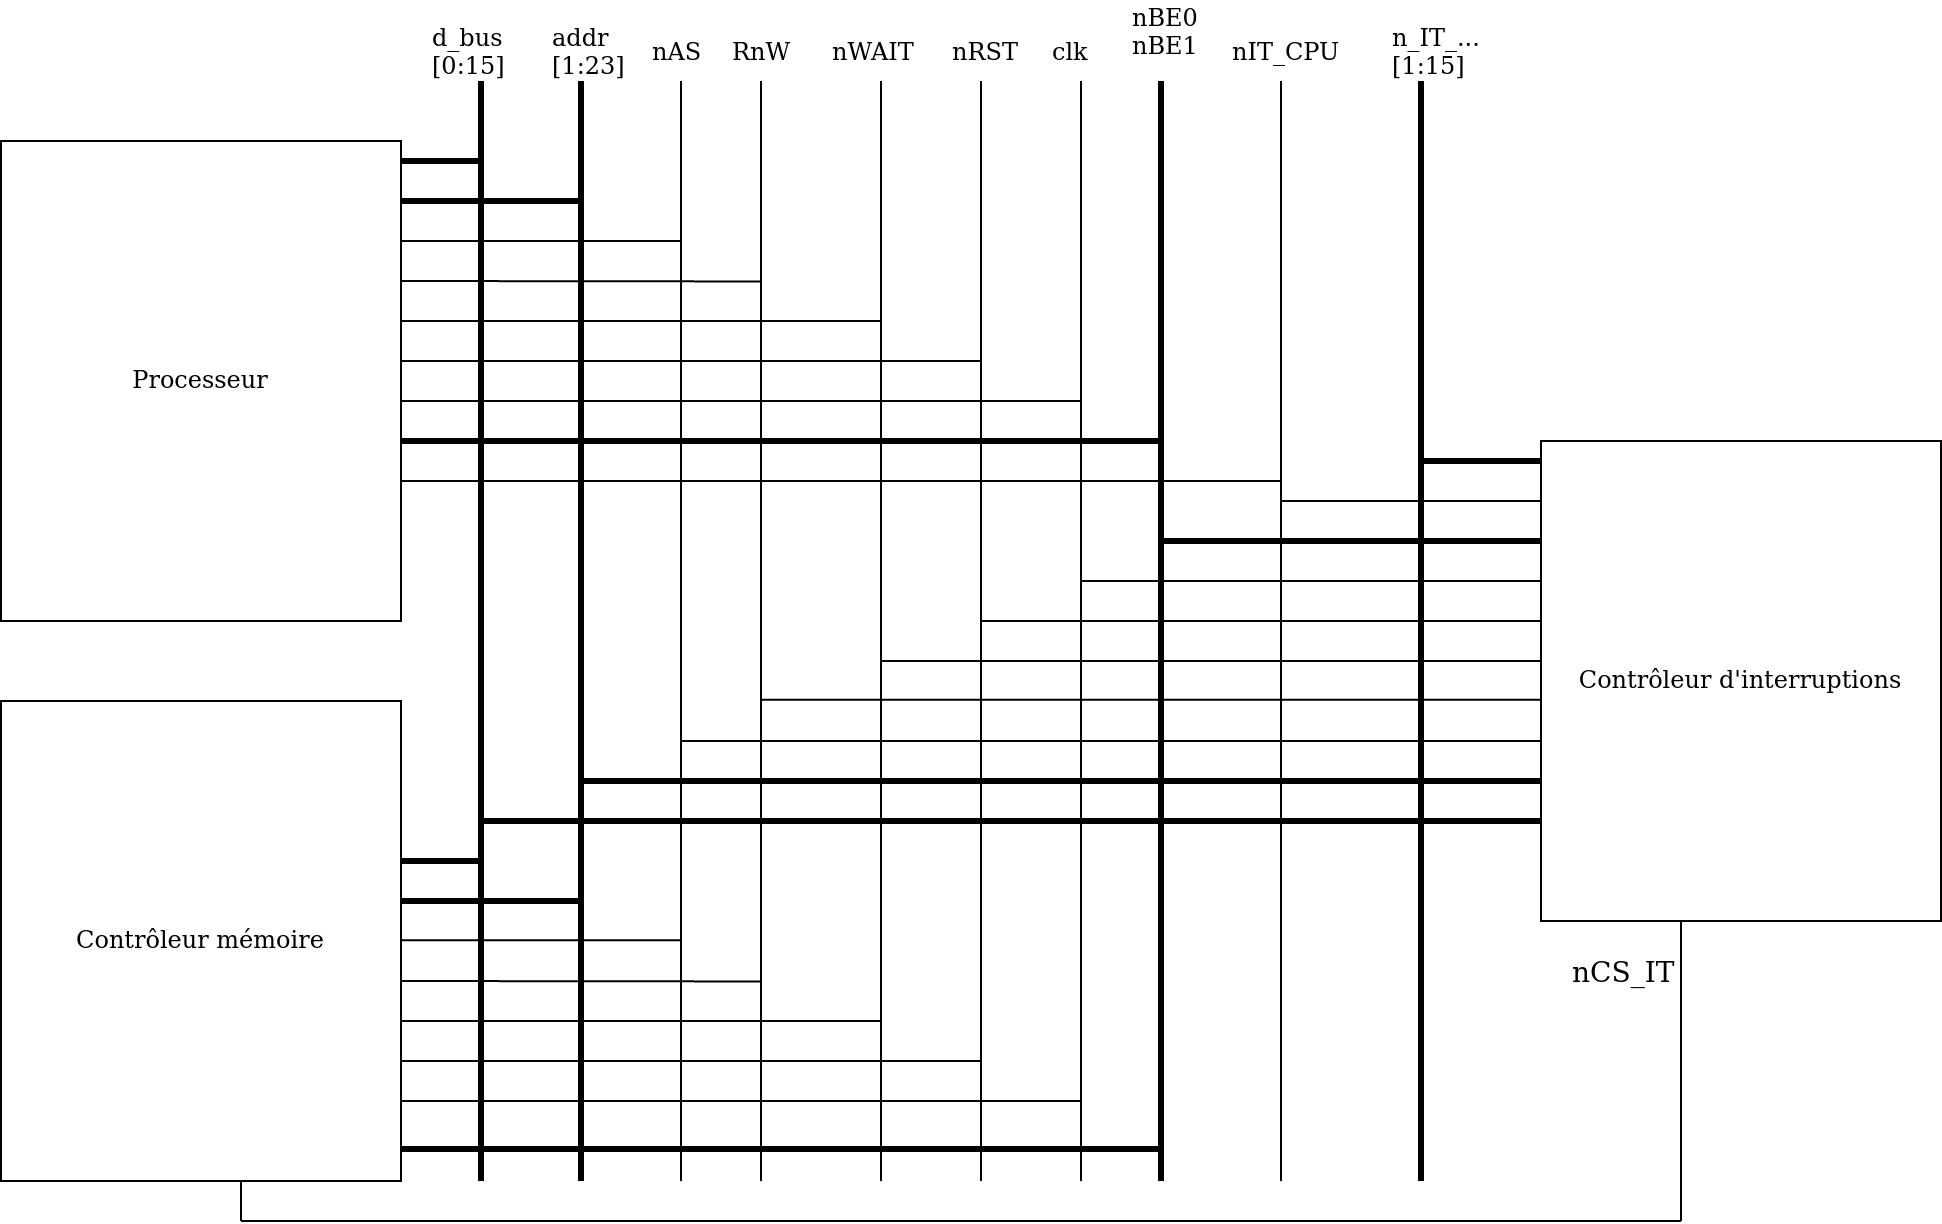
\includegraphics[width=1\linewidth]{figure/schema_cablage.png}
	\caption{Schéma de câblage de l'IP à concevoir, du contrôleur mémoire et du processeur}
	\label{fig:schema_cablage}
\end{figure}
	
Le contrôleur d'interruptions est également câblé avec plusieurs autres IPs du SoC.
Il y a par exemple le processeur avec lequel le signal nIT\_CPU est commun.
D'autre part le contrôleur mémoire est connecté avec le contrôleur d'interruptions par le signal nCS\_IT. L'ensemble des périphériques du SoC peut également envoyer un signal d'interruption représenté par nIT\_ $\dots$\\
	
Le schéma présenté ci-dessus ne précise pas le sens des signaux.
Il n'est donc pas possible de savoir quelles sont les entrées et sorties du contrôleur d'interruptions.
Également, les noms des 4 interruptions externes et des 11 autres provenant de divers périphériques ne sont pas donnés.
La figure \ref{fig:spe_bus} et le tableau \ref{tab:sens_role_signaux} présentent les entrées et sorties du point de vue de l'IP à concevoir ainsi que le rôle de chaque signaux. 
	
\begin{figure}[H]
	\centering
	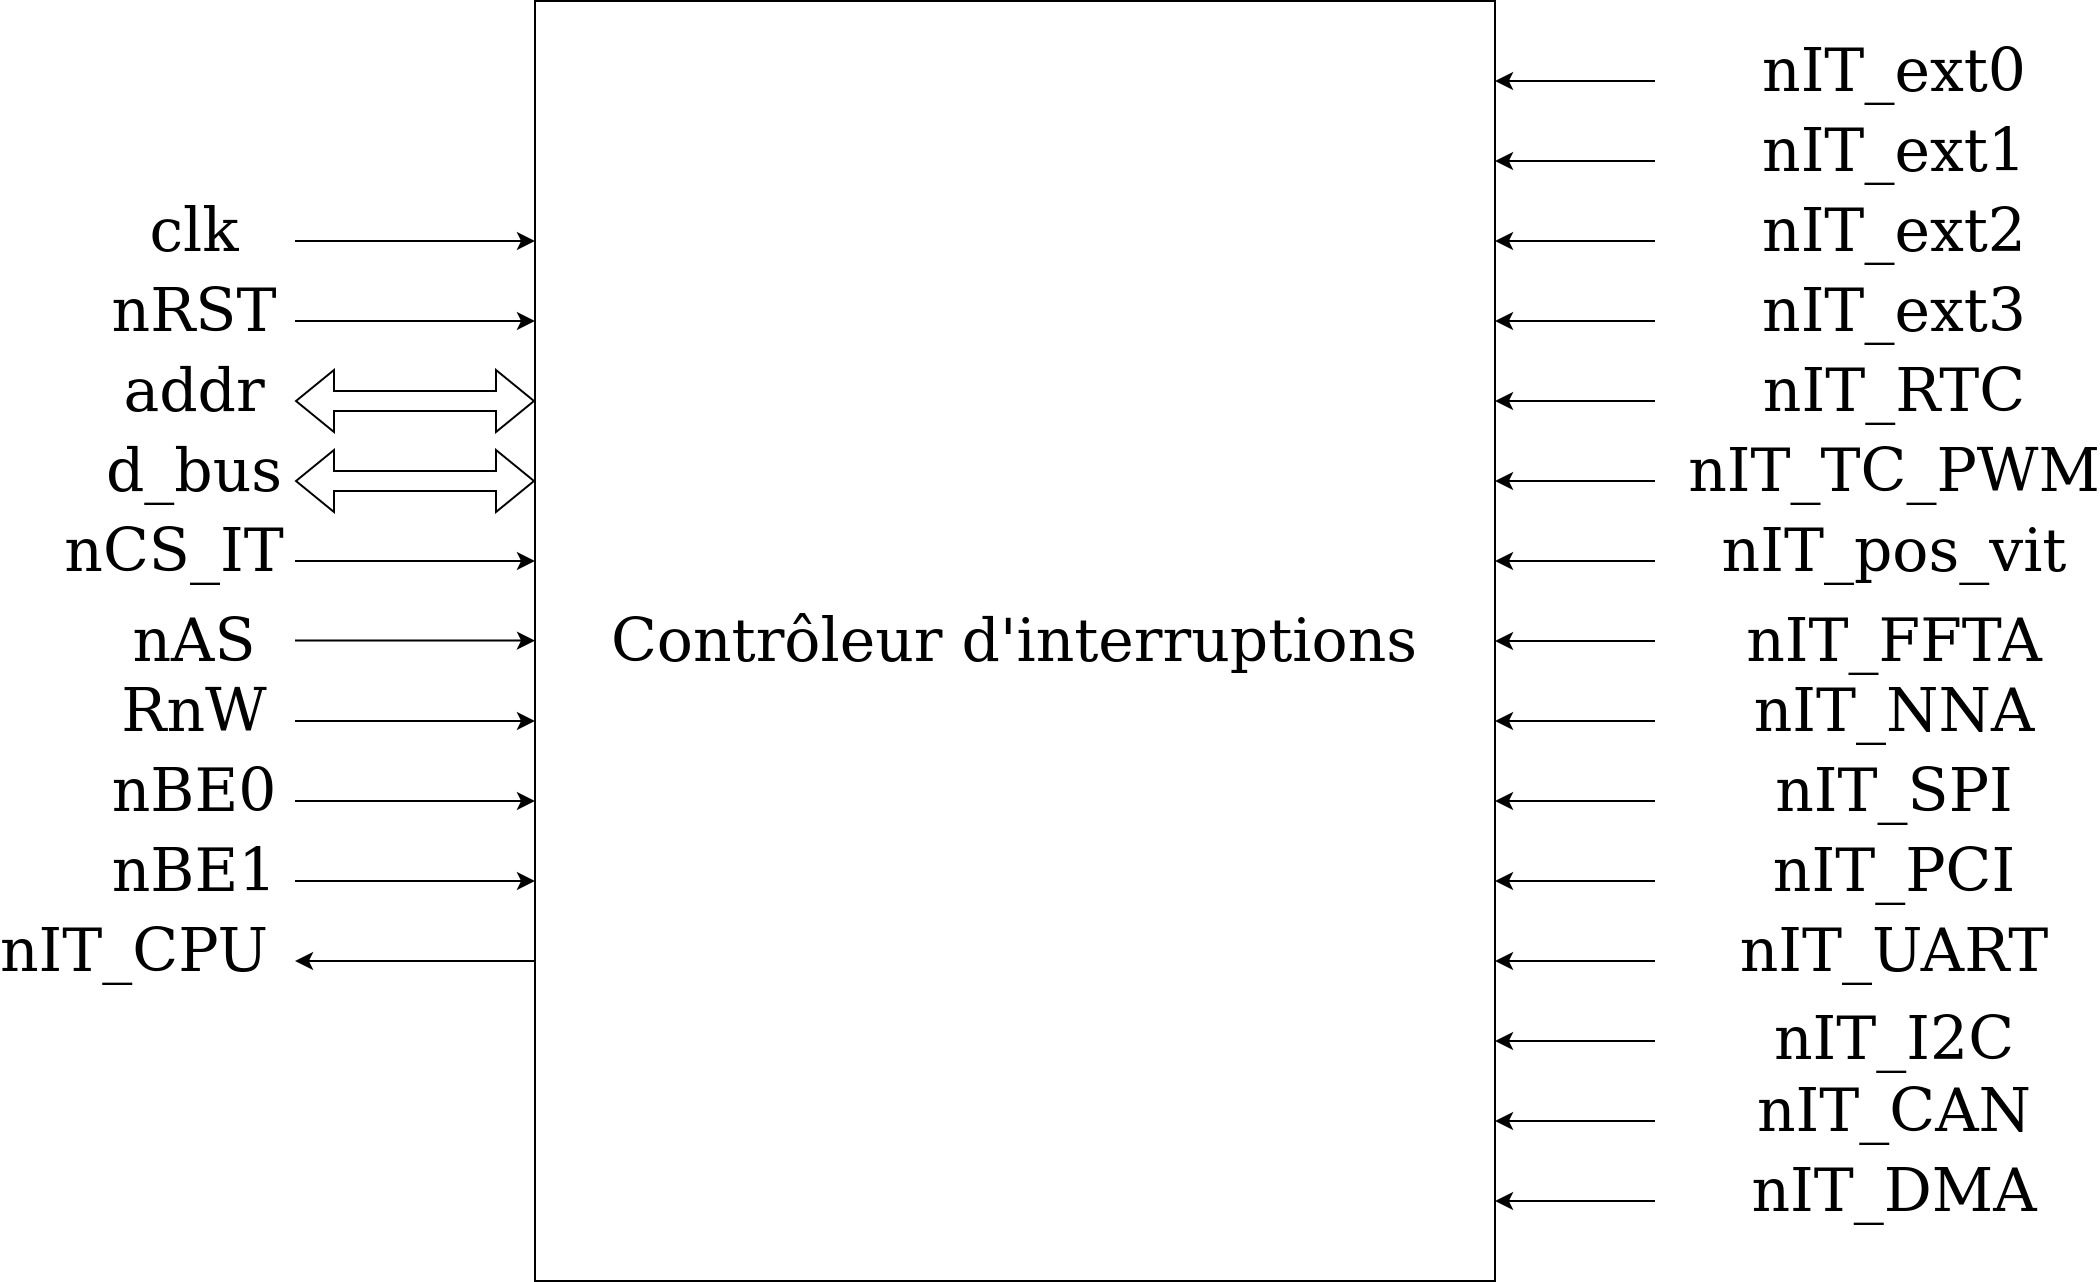
\includegraphics[width=0.8\linewidth]{figure/delimitation_systeme.png}
	\caption{Entrées et sorties de l'IP à concevoir}
	\label{fig:inout_ip}
\end{figure}


\begin{table}[H]
	\centering
	\begin{tabular}{|c|c|c|}
		\hline
		Nom & Sens & Rôle\\
		\hline
		clk & Entrée & Signal d'horloge\\
		\hline
		nRST & Entrée & Signal de réinitialisation\\
		\hline
		addr & Entrée et sortie & Bus d'adresses\\
		\hline
		d\_bus & Entrée et sortie & Bus de données\\
		\hline
		nCS\_IT & Entrée & Signal de sélection du périphérique en cas \\
		& & d'opérations de lecture ou d'écriture\\
		\hline
		nAS & Entrée & Signal indiquant la présence d'une valeur\\
		& & sur le bus d'adresse\\
		\hline
		& & Signal d'écriture ou de lecture\\
		RnW & Entrée & 0 : écriture\\
		& & 1 : lecture\\
		\hline
		 & & Signal indiquant la structure de la mémoire\\
		nBE0 & Entrée & 0 : little-endian\\
		& & 1 : big-endian\\
		\hline
		& & Signal indiquant la taille de la donnée\\
		nBE1 & Entrée & 0 : 8 bits\\
		 & & 1 : 16 bits\\
		\hline
		 &  & Signal pour le processeur avertissant \\
		nIT\_CPU & Sortie & qu'une interruption est demandée de la part d'un \\
		& & périphérique\\
		\hline
		nIT\_ext0 & Entrée & Signal d'interruption extérieure numéro 0\\
		\hline
		nIT\_ext1 & Entrée & Signal d'interruption extérieure numéro 1\\
		\hline
		nIT\_ext2 & Entrée & Signal d'interruption extérieure numéro 2\\
		\hline
		nIT\_ext3 & Entrée & Signal d'interruption extérieure numéro 3\\
		\hline
		nIT\_RTC & Entrée & Signal d'interruption provenant du périphérique RTC\\
		\hline
		nIT\_TC\_PWM & Entrée & Signal d'interruption provenant du Timer et PWM\\
		\hline
		nIT\_pos\_vit & Entrée & Signal d'interruption provenant du\\
		& & périphérique de mesure position et vitesse\\
		\hline
		nIT\_FFTA & Entrée & Signal d'interruption provenant de \\
		& & l'accélérateur transformée de Fourier discrète\\
		\hline
		nIT\_NNA & Entrée & Signal d'interruption provenant de \\
		& & l'accélérateur réseau de neurones\\
		\hline
		nIT\_SPI & Entrée & Signal d'interruption provenant du \\
		& & périphérique de communication SPI\\
		\hline
		nIT\_PCI & Entrée & Signal d'interruption provenant du \\
		& & périphérique de communication PCI\\
		\hline
		nIT\_UART & Entrée & Signal d'interruption provenant du \\
		& & périphérique de communication UART\\
		\hline
		nIT\_I2C & Entrée & Signal d'interruption provenant du \\
		& & périphérique de communication I2C\\
		\hline
		nIT\_CAN & Entrée & Signal d'interruption provenant du \\
		& & périphérique de communication CAN\\
		\hline
		nIT\_DMA & Entrée & Signal d'interruption provenant du \\
		& & périphérique d'accès direct à la mémoire.\\
		\hline
	\end{tabular}
	\caption{Sens et rôle des signaux}
	\label{tab:sens_role_signaux}
\end{table}
	
Les noms des signaux présentent un suffixe n signifiant que ceux-ci sont actifs à l'état bas.
Par exemple, le signal de sélection nCS\_IT est actif à l'état bas.
Ainsi un signal de sélection à l'état logique 0 signifie que le contrôleur d'interruptions est sélectionné pour une opération de lecture ou d'écriture dans un des registres.


Conventionner ces signaux comme actif à l'état bas n'est pas anodin.
Historiquement, pour des anciennes technologies \gls{TTL}, les signaux actifs à l'état bas sont davantage robustes aux bruits.  
À titre d'exemple, un signal de sélection CS actif à l'état haut sélectionne un périphérique lorsque celui-ci est à l'état logique 1.
Pour des raisons purement physiques (glitch sur le signal, baisse de tension à cause de la résistivité des interconnexions, chute de l'alimentation à cause d'un fort tirage de courant), ce signal à l'état 1 peut passer à l'état de haute impédance Z, voire à l'état bas.
Un tel problème causerait la perdre de données à lire où écrire mais plus généralement des problèmes de sécurité. 


\subsection{Chronogrammes caractéristiques}
Cette partie détaille les contraintes temporelles via à vis des entrées sorties. 
Il est possible d'identifier deux types d'échanges pour ce périphérique.
Le premier via le bus est illustré avec le chronogramme figure \ref{fig:spe_bus}.
\begin{figure}[H]
	\centering
	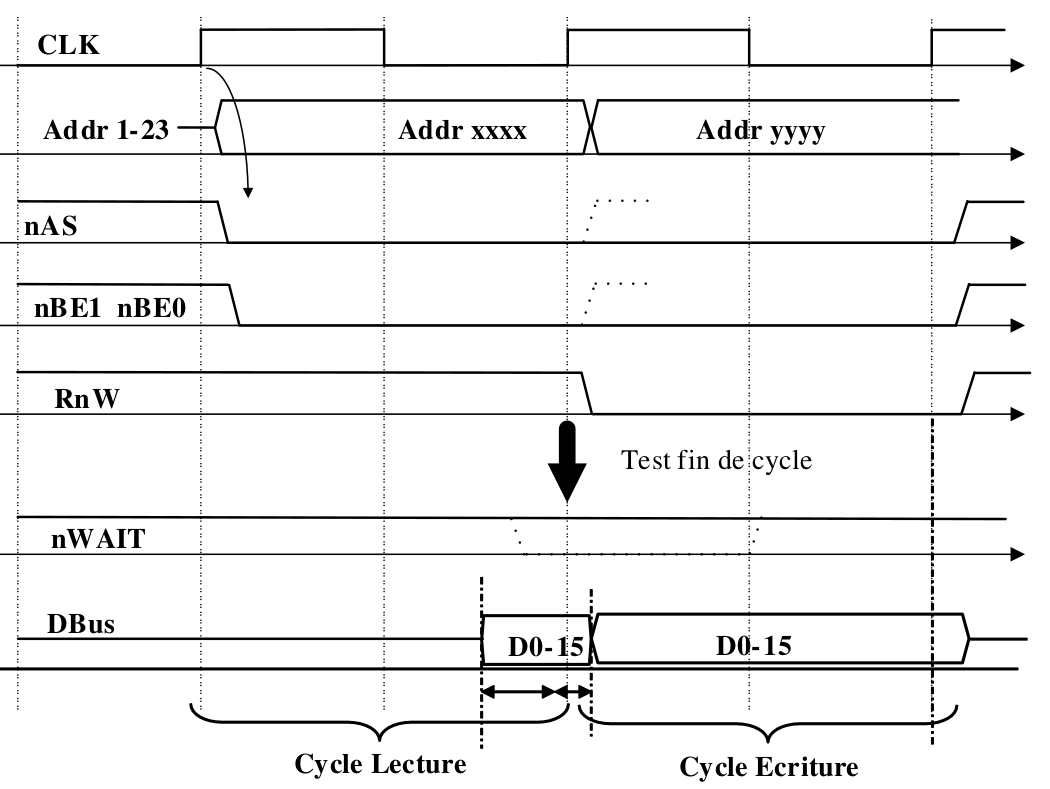
\includegraphics[width=0.7\linewidth]{chrono_specif_bus.png}
	\caption{Chronogramme spécification du bus}
	\label{fig:spe_bus}
\end{figure}
On retrouve une partie des signaux définis dans la figure \ref{fig:inout_ip}. 
Lors du premier front d'horloge une valeur est placée sur le bus d'adresse comme l'indique sa valeur et nAS. 
Le périphérique doit alors lire ou écrire la valeur correspondante sur le bus de données avant le prochain front montant. 
C'est ce qu'indique la flèche centrale sur cette figure. 
Respecter cette contrainte permettra d'assurer la compatibilité entre les entités communiquant sur le bus.
Ce dernier permet un échange bidirectionnel entre le processeur et le contrôleur.
Il servira à accéder par lecture et écriture aux différents registres.
Parmi eux, on identifie le vecteur d'exception qui sauvegarde les adresses mémoire auxquelles le processeur va brancher.
Le registre de masquage permettra de désactiver individuellement chaque entrée.
La priorité par défaut de chaque entrée pourra également être modifiée.

\gap
Le second type de communication a pour but de notifier le \gls{CPU} lors d'interruptions.
Elles peuvent provenir des autres périphériques présents dans le microcontrôleur ou de sources externes.
L'objectif est d'informer le processeur via le signal nIT\_CPU en suivant le régime de priorités.
\begin{figure}[H]
	\centering
	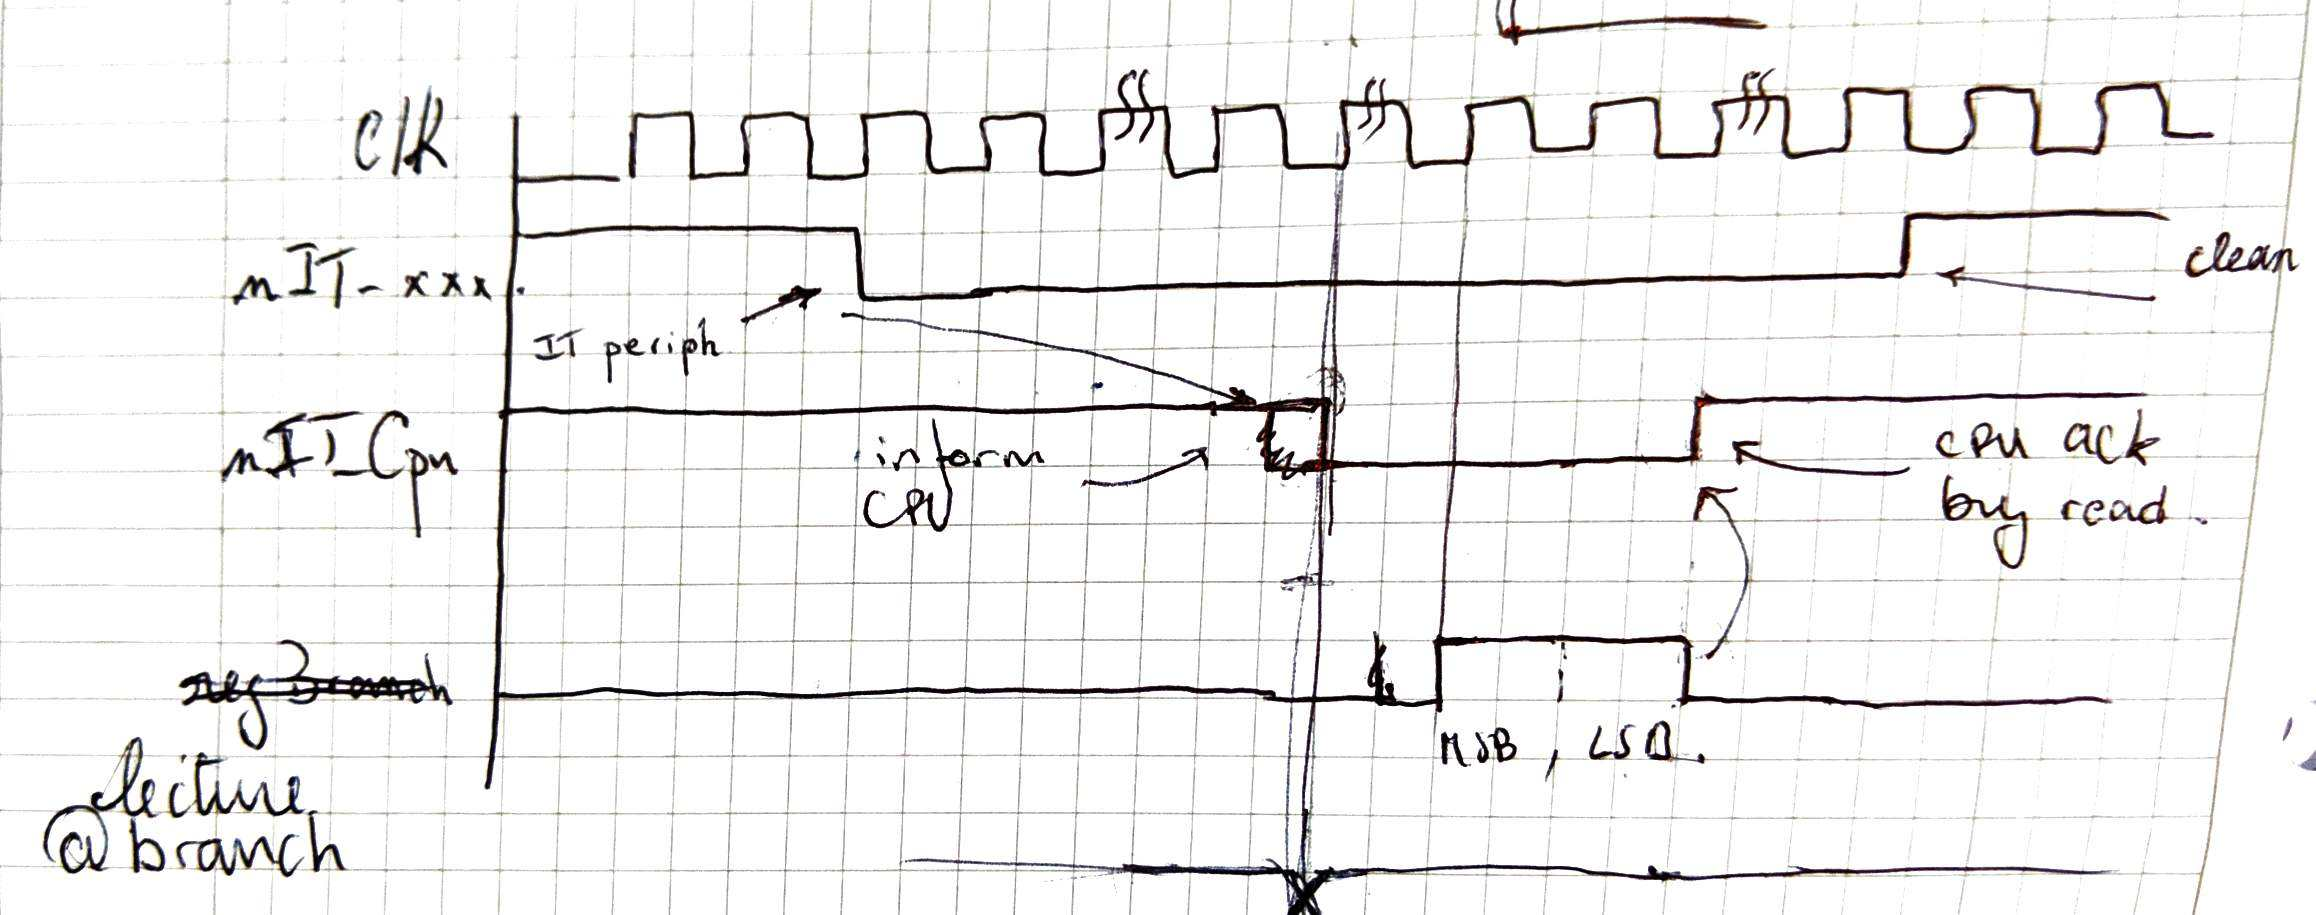
\includegraphics[width=0.7\linewidth]{chrono_specif_IT.png}
	\caption{Chronogramme spécification signal IT au processeur}
	\label{fig:spe_IT}
\end{figure}
Le chronogramme figure \ref{fig:spe_IT} illustre le cas d'un signal d'interruption provenant d'un périphérique et la séquence induite concernant le signal nIT\_CPU.
Une demande d'interruption s'identifie par un front descendant de nIT\_xxx. 
Après quelques cycles de traitement visant à confirmer la validité de la requête en consultant le registre de masquage, le processeur est informé, lui aussi, par un front descendant sur nIT\_CPU.
Il sauvegarde alors le contexte et lit le registre de branchement.
Cette action agit comme un \textbf{acquittement} et le signal nIT\_CPU est passé à l'état bas.
Le processeur se charge d'informer le périphérique émetteur, souvent à la fin de la routine, afin qu'il baisse le drapeau dans son registre d'état.
Tant que cela n'est pas fait, aucune demande d'interruption de niveau inférieur ou égal ne sera transmis.
Le chronogramme figure \ref{fig:spe_IT} illustre justement le cas d'une demande \textbf{moins prioritaire} qui apparaît durant l'exécution d'une première.
\begin{figure}[H]
	\centering
	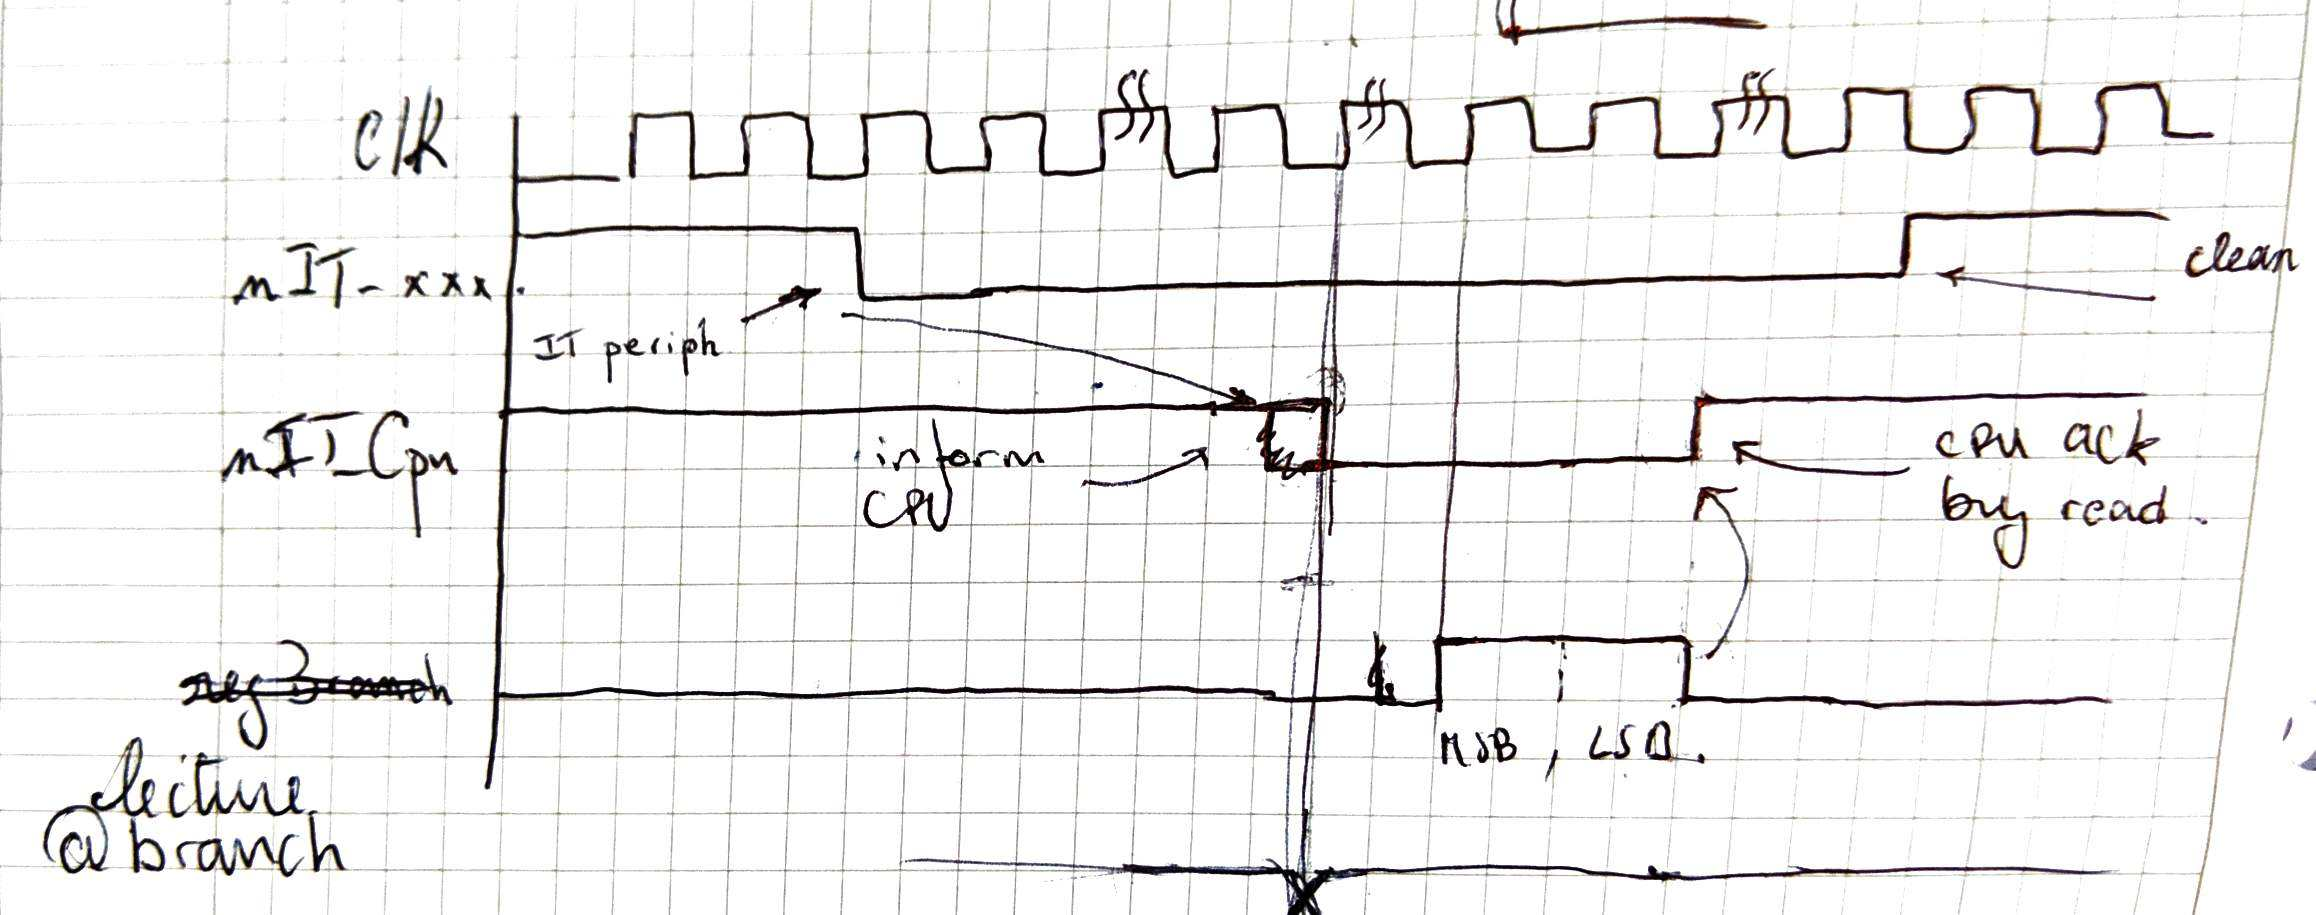
\includegraphics[width=0.7\linewidth]{chrono_specif_IT.png}
	\caption{Chronogramme spécification 2 signaux IT cas 1}
	\label{fig:spe_IT}
\end{figure}
Dans cette situation, le périphérique d'indice 1 est plus prioritaire que celui d'indice 2. 
La demande est faite comme précédemment en passant le signal nIT\_xx1 à l'état bas.
Le contrôleur réagit alors en informant le processeur.
Pendant cette opération, une seconde interruption de niveau inférieur apparaît.
Aucune réaction n'est attendu de la part du contrôleur qui attend la fin de l'exécution précédente pour générer un front descendant sur nIT\_CPU.
Le traitement se déroule alors comme auparavant.
Il est intéressant de porter l'attention sur la place que joue le signal nIT\_xx1 dans ce cas.
Son passage à l'état haut autorise de nouveau l'occurrence des interruptions de niveau inférieur ou égal.
Il reviendra donc au développeur de placer cet acquittement en fin de routine d'interruption sans quoi la priorisation ne sera pas garantie.
Pour poursuivre la description des contraintes temporelles, on peut identifier un second cas venant de paire avec le précédent.
Le chronogramme figure \ref{fig:spe_2IT} illustre la situation où une demande \textbf{plus prioritaire} apparaît durant l'exécution d'une première.
\begin{figure}[H]
	\centering
	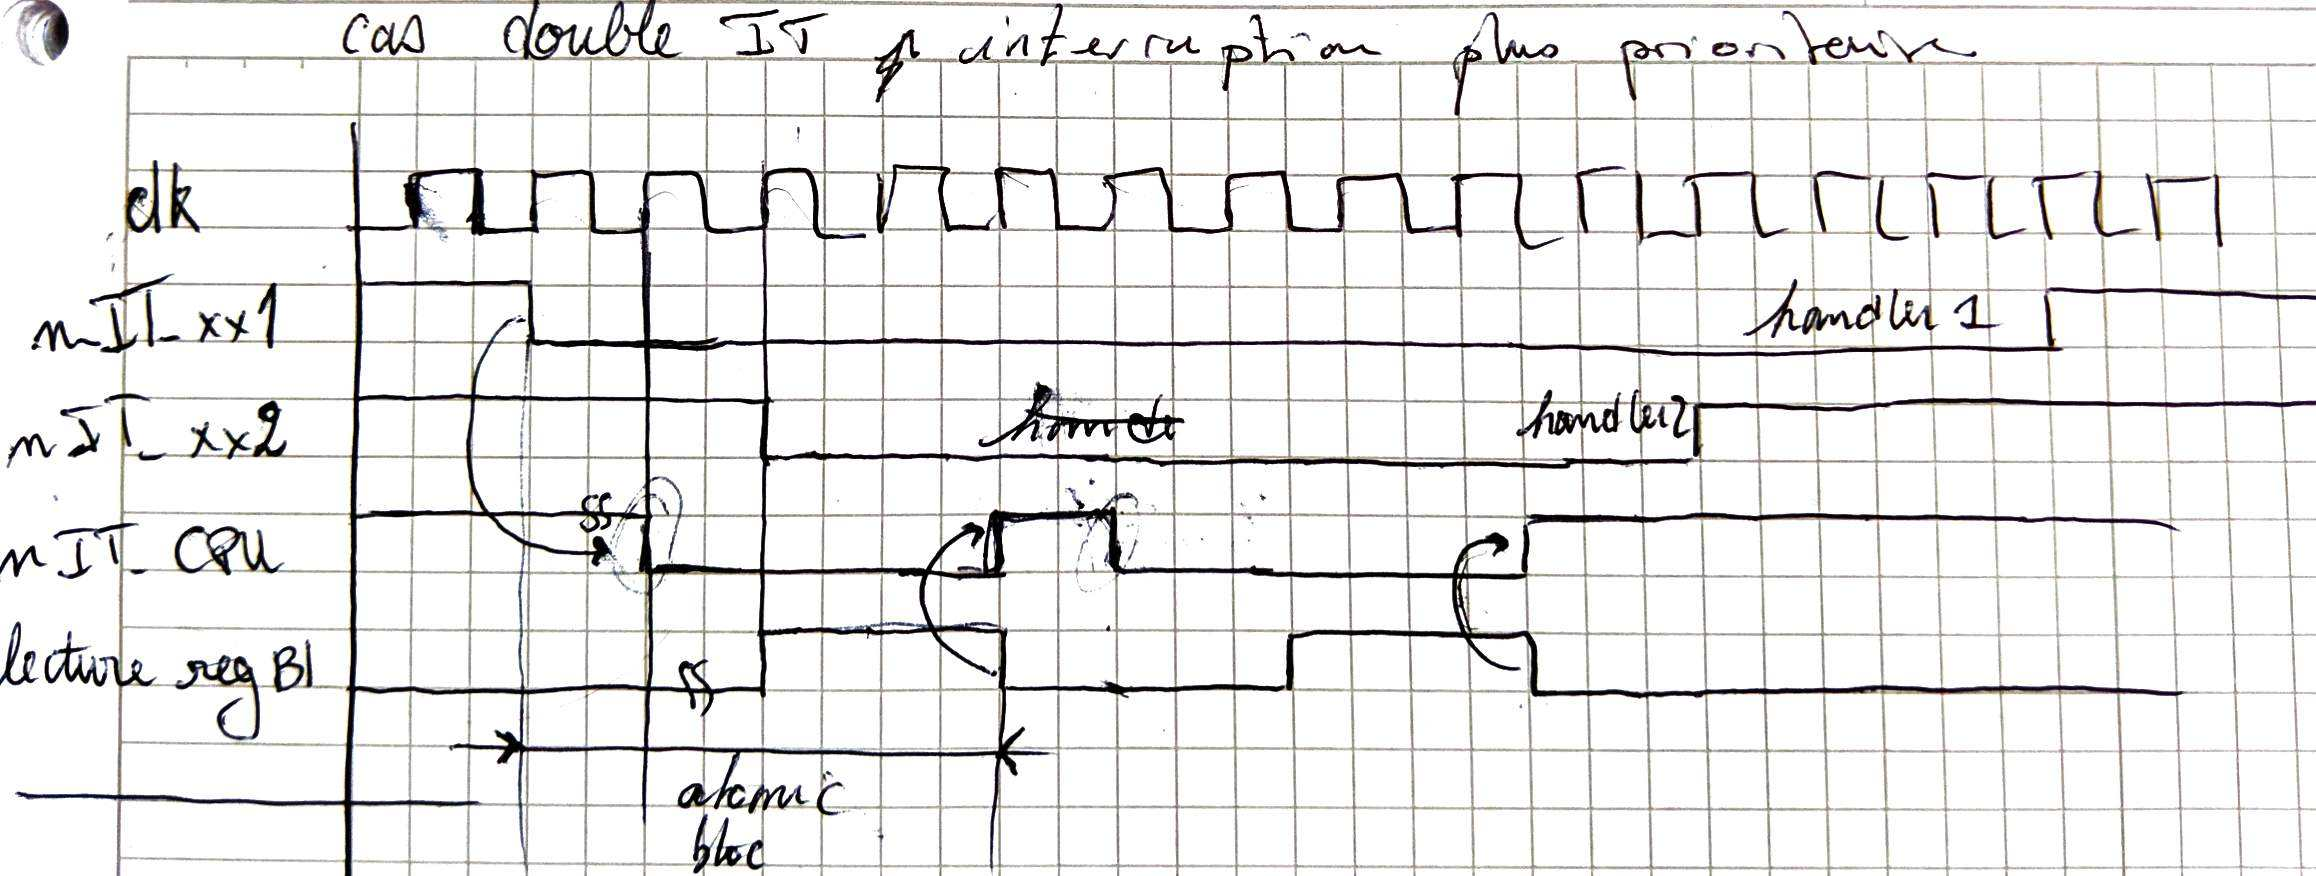
\includegraphics[width=0.7\linewidth]{chrono_specif_2IT.jpg}
	\caption{Chronogramme spécification 2 signaux IT cas 2}
	\label{fig:spe_2IT}
\end{figure}
De nouveau, dans ce cas, le périphérique d'indice 1 est plus prioritaire que celui d'indice 2. 
Une première demande provient du signal nIT\_xx2.
Mais durant son traitement, il apparaît, une seconde interruption de niveau supérieur.
Le contrôleur attend alors la lecture du processeur pour la première avant de l'informer pour la seconde.
Cela est primordial pour éviter toute incohérence dans l'état des registres.
Lorsque le processeur a effectué la lecture servant d'acquittement, il est de nouveau notifié.
Le signal nIT\_CPU doit alors rester au minimum un cycle horloge à l'état bas afin de générer un front descendant synchrone.
La suite du cycle se passe comme précédemment pour le contrôleur d'IT.
C'est le processeur qui gère le rétablissement du contexte de l'interruption de plus faible priorité.

\gap
Nous venons de présenter trois situations de gestion d'interruptions. 
Cette analyse est loin d'être exhaustive, principalement en raison de l'infinité des instants d'occurrence possibles.
Il semble toutefois que les cas traités couvrent l'ensemble des séquences d'événements.
Pour vérifier la conformité d'un cas quelconque, il sera alors possible de s'y référer en identifiant la situation et en adaptant l'échelle temporelle.

\subsection{Contraintes du projet}

La section qui suit traite de la gestion du projet.
Il s'agit de préciser la planification du projet avec des divers livrables à fournir à des dates précises.
La figure (\ref{fig:planning}) ci-dessous est le plan de développement du projet.
Les losanges bleus sont les jalons à fournir.
La conception de cet IP a débuté le 5 octobre 2022 c'est-à-dire à la 40$^{\mbox{ème}}$ semaine de l'année.
Le rendu de l'IP et du rapport de conception s'effectuera la semaine 49.

\begin{figure}[H]
	\centering
	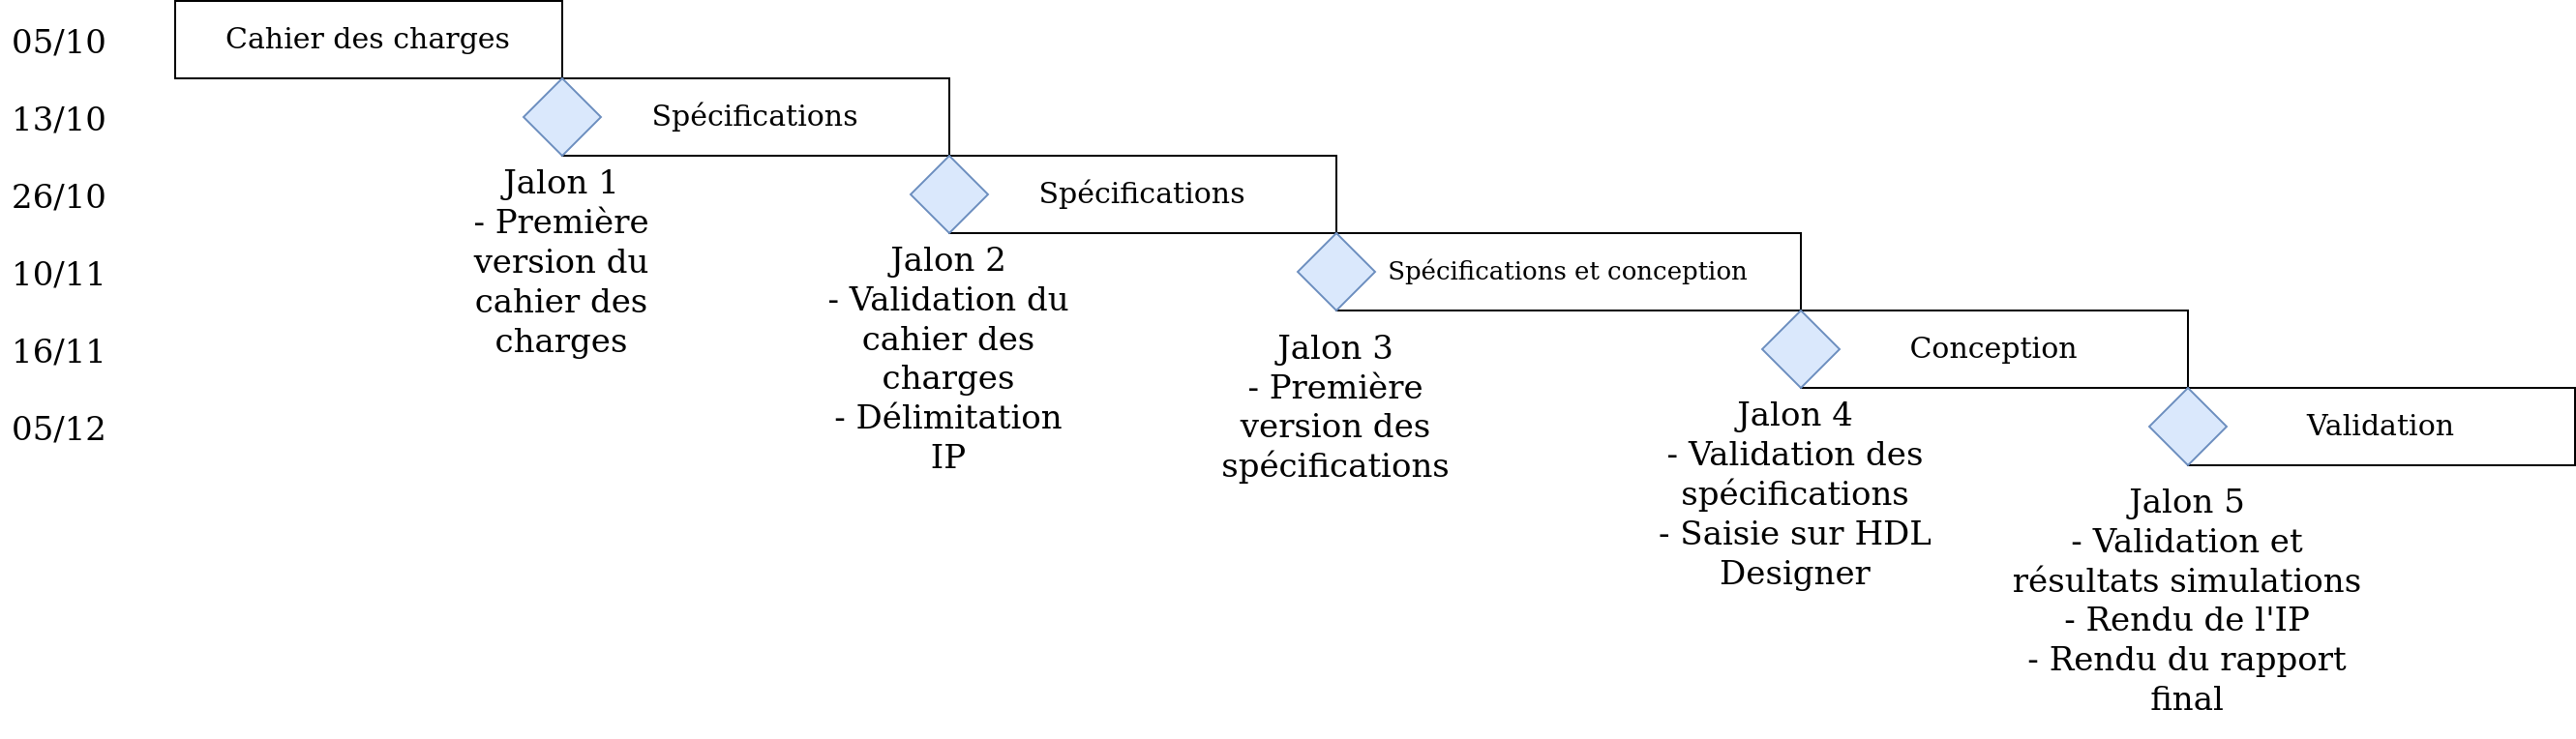
\includegraphics[width=1\linewidth]{figure/planning.png}
	\caption{Planification du projet avec ses jalons}
	\label{fig:planning}
\end{figure}

Également, le projet est contraint d'un point de vue ressources disponibles.
La liste suivante présente les ressources attribuées pour la conception de ce contrôleur d'interruptions.

\begin{itemize}
	\item 2 concepteurs
	\item Outils EDA de Mentor Graphics (propriété de Siemens EDA)
	\item Carte d'évaluation ZYNQ-7 basé sur un FPGA Zynq-7000
\end{itemize}
